\section{Generalized Coordinates}
\label{sect:generalized-coordinates}

Given a greedily realizable sequence of simple paths ${\Pi = (P_1, \ldots, P_k)}$, we shall now choose generalized coordinates such that the holonomic constraints defined by ${\Pi}$ are implicitly satisfied. The generalized coordinates introduced here require a circular arc's endpoints to differ and can therefore not be applied to paths whose endpoints coincide.

\hfill

\noindent
Besides its endpoints, a circular arc requires another generalized coordinate encoding its curvature for it to be uniquely determined. This coordinate must be able to encode the arc's direction, \ie{} whether it is drawn clockwise or counterclockwise. Considering two circular arcs with the same angle $\varphi$, as introduced in the previous section, are guaranteed to be similar, we shall use the angle ${\varphi_P \in (-180 \degrees, 180 \degrees)}$ as a generalized coordinate encoding the curvature of the circular arc ${\Gamma_P}$.

Unconstrained vertices ${v \in V_\text{u}(\Pi)}$ can move around arbitrarily and require two degrees of freedom. We shall use Cartesian coordinates ${(x_v, y_v) \in \mathbb{R}^2}$ to represent their positions.

In contrast, constrained vertices ${v \in V_\text{c}(\Pi)}$ can not move around arbitrarily \emdash they are each being laid out by a path ${P(v)}$ and are restricted to move along the circular arc ${\Gamma_{P(v)}}$, while also staying in the order indicated by ${P(v)}$. We only have one degree of freedom per vertex here: its relative progress along the arc. It can be encoded using a generalized coordinate ${p_v \in (0, 1)}$ specifying the proportion of the subarc connecting ${P(v)}$'s tail and ${v}$ to the entire arc, as illustrated in \cref{fig:generalized-coordinates-for-single-path}.



\hfill
\begin{figure}[H]
  \centering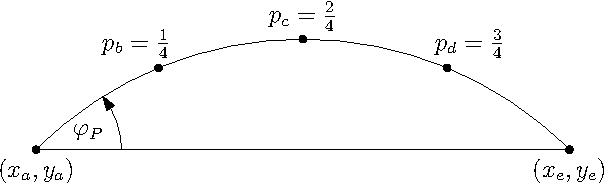
\includegraphics[width=0.7\textwidth]{Resources/Figures/Generalized-Coordinates-Example.pdf}
  \caption{Generalized coordinates for a single path ${P = abcde}$ with equi-length edges.}
  \label{fig:generalized-coordinates-for-single-path}
\end{figure}
\clearpage



\noindent
Collectively, the ${\bigTheta{\abs{V} + \abs{\Pi}}}$ generalized coordinates uniquely determine all of the vertices' positions ${\vec{r}_v}$ and circular arcs ${\Gamma_P}$. We shall write them as a 4-tuple ${q_{_\Pi} = (x, y, \varphi, p)}$, where
%
\begin{alignat*}{3}
  x & \colon & V_\text{u}(\Pi) &\to \mathbb{R},\\
  y & \colon & V_\text{u}(\Pi) &\to \mathbb{R},\\
  \varphi & \colon & \phantom{V_\text{u}(}\Pi\phantom{)} &\to (-180 \degrees, 180 \degrees),\\
  p & \colon & V_\text{c}(\Pi) &\to (0, 1).
\end{alignat*}

\noindent
The generalized coordinates chosen here satisfy all holonomic constraints defined by ${\Pi}$, \ie{} all vertices ${v \in V(P)}$ on a path ${P \in \Pi}$ are guaranteed to lie on the same circular arc $\Gamma_P$.

Recall that the configurations that can be expressed only depend on the constraints implicitly satisfied by the choice of generalized coordinates, and that the number of independent generalized coordinates equals the number of degrees of freedom in the system. It is therefore not possible to use fewer generalized coordinates while satisfying the same constraints without also excluding other configurations.
